\section{Code Examples}

\subsection{Sorting}
\begin{frame}{Sorting}
    \begin{columns}
    \column{0.6\textwidth}
        \begin{itemize}
            \item percentageFullMatch = Percentage Full Match
            \item percentagePartialMatch = Percentage Partial Match
            \item getRating = Rating
            \item prevIngredients = Previous Ingredients
            \item recipe.Title = Recipe Title
        \end{itemize}
    \column{0.4\textwidth}
        \begin{figure}
            \centering
            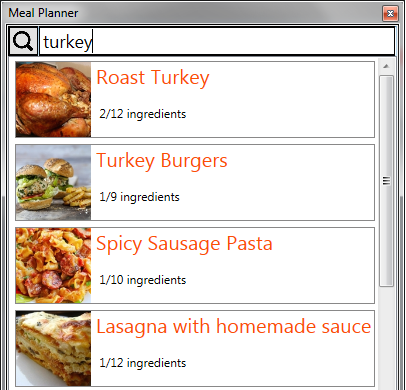
\includegraphics[width=\textwidth]{graphics/recipe-search-item}
        \end{figure}
    \end{columns}

\end{frame}

\subsection{PublicQuerys}
\begin{frame}{PublicQuerys}
    \begin{itemize}
        \item IQueryable<inventoryListGroupedByQuantity> inventoryIQueryable
        \item List<inventoryListGroupedByQuantity> inventoryList
        \item List<LastMeal> ingredientsFromLastMeals
        \item List<int> blackList
        \item List<GrayList> grayList
    \end{itemize}
\end{frame}

%\begin{frame}{Search by recipes}
    %\begin{figure}
        %\centering
        %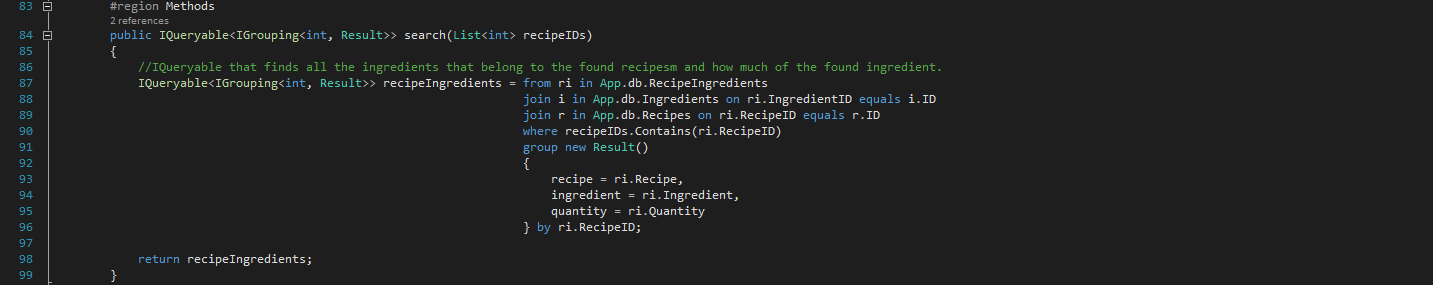
\includegraphics[width=\textwidth]{Grafik/search}
    %\end{figure}
%\end{frame}

\subsection{Sorting Of Results}
\begin{frame}[fragile]{Sorting Of Results}{Initialize result}
\begin{lstlisting}
public ObservableCollection<SearchResults> addValuesToSearch(IQueryable<IGrouping<int, Result>> userInput, List<string> searchKeywords = null)
{
    ObservableCollection<SearchResults> result = new ObservableCollection<SearchResults>();

    foreach (IGrouping<int, Result> ri in userInput)
    {
        Recipe recipe = ri.FirstOrDefault().recipe;

        SearchResults searchResult = new SearchResults(recipe);
\end{lstlisting}
\end{frame}

\begin{frame}[fragile]{Sorting Of Results}{Check Recipe For Keyword}
\begin{lstlisting}
if (searchKeywords != null)
{
    if (searchKeywords.Any(s => recipe.Title.ToLower().Contains(s.ToLower())))
    {
        searchResult.keyWordMatch++;
    }
}
foreach (Result res in ri)
{
    searchResult.addIngredient(res.ingredient);
\end{lstlisting}
\end{frame}

\begin{frame}[fragile]{Sorting Of Results}{Check inventory}
\begin{lstlisting}
if (inventoryList.Where(il => il.IngredientID == res.ingredient.ID).Count() != 0)
{
    if (inventoryList.Where(il => il.IngredientID == res.ingredient.ID).First().Quantity >= res.quantity)
    {
        searchResult.fullMatch++;
    }
    else
    {
        searchResult.partialMatch += inventoryList.Where(il => il.IngredientID == res.ingredient.ID).First().Quantity / res.quantity;
    }
}
\end{lstlisting}
\end{frame}

\begin{frame}[fragile]{Sorting Of Results}{Check Ingredient For Keyword}
\begin{lstlisting}
if (searchKeywords != null)
{
    if (searchKeywords.Any(s => res.ingredient.Name.ToLower().Contains(s.ToLower())))
    {
        searchResult.keyWordMatch++;
    }
}
\end{lstlisting}
\end{frame}

\begin{frame}[fragile]{Sorting Of Results}{Check Ingredient In Last Meals}
\begin{lstlisting}
if (ingredientsFromLastMeals.Where(iflm => iflm.ingredientID == res.ingredient.ID).Count() != 0)
{
    searchResult.prevIngredients += ingredientsFromLastMeals.Where(iflm => iflm.ingredientID == res.ingredient.ID).Single().ingredientCount;
}
\end{lstlisting}
\end{frame}

\begin{frame}[fragile]{Sorting Of Results}{Check Ingredient On Graylist}
\begin{lstlisting}
if (grayList.Where(gl => res.ingredient.ID == gl.ingredient.ID).Count() != 0)
{
    searchResult.setRating = grayList.Where(gl => res.ingredient.ID == gl.ingredient.ID).SingleOrDefault().rating;
}
else
{
    searchResult.setRating = 50;
}
\end{lstlisting}
\end{frame}

\begin{frame}[fragile]{Sorting Of Results}{Ordering And Returning Results}
\begin{lstlisting}
    result.Add(searchResult);
}

return new ObservableCollection<SearchResults>(result.OrderByDescending(res => res.percentageFullMatch).ThenByDescending(res => res.percentagePartialMatch).ThenByDescending(res => res.getRating).ThenByDescending(res => res.prevIngredients).ThenByDescending(res => res.recipe.Title));
\end{lstlisting}
\end{frame}




















